\uuid{MLRe}
\exo7id{7270}
\auteur{mourougane}
\organisation{exo7}
\datecreate{2021-08-10}
\isIndication{false}
\isCorrection{false}
\chapitre{Géométrie affine euclidienne}
\sousChapitre{Géométrie affine euclidienne du plan}

\contenu{
\texte{
Le \emph{théorème de Bolyai} affirme que deux polygones de même aire peuvent toujours être obtenus 
l'un à partir de l'autre par découpage et recollement.
On va étudier le découpage d'un triangle équilatéral pour obtenir un carré de même aire.


\textit{On considère un triangle équilatéral $ABC$ que l'on souhaite découper de façon à pouvoir le transformer en un rectangle, voire un carré.}

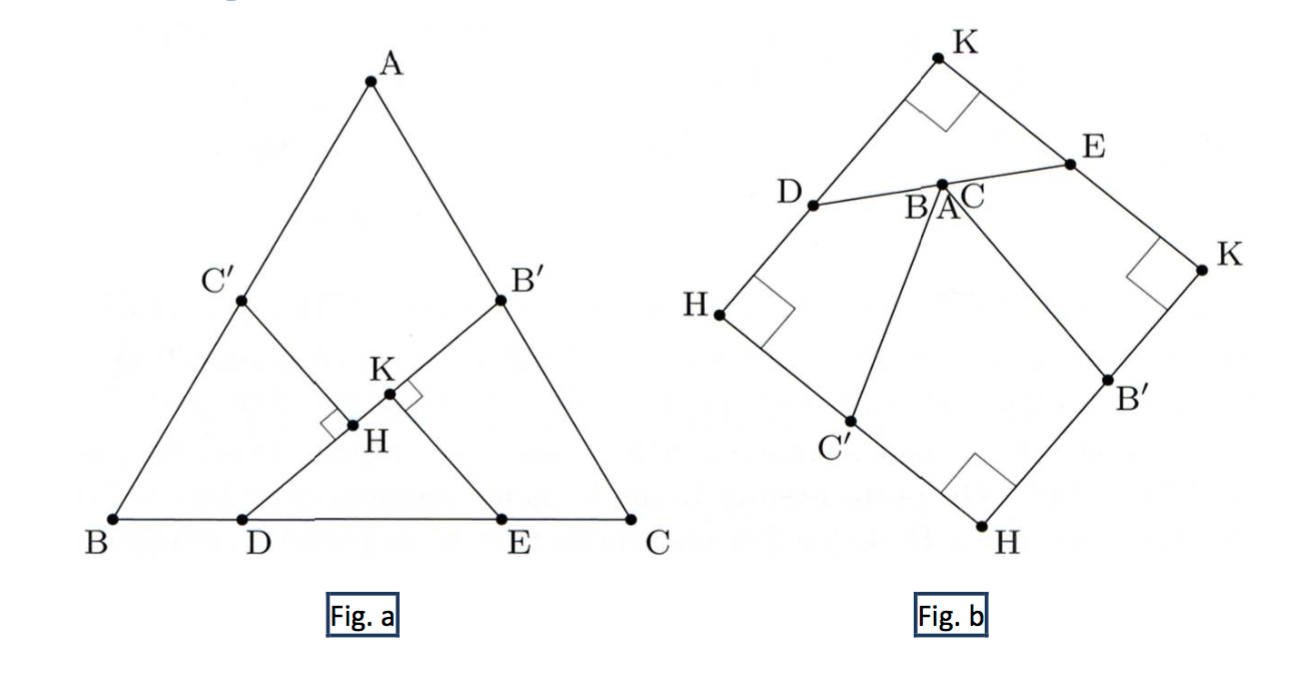
\includegraphics[scale=0.6]{images/img-mour-022-1}
}
\begin{enumerate}
    \item \question{On part du triangle équilatéral $ABC$ et on place un point $D$ sur $[BC]$ tel que $0<BD<\frac{1}{2}BC$. On construit ensuite $E$ sur le même segment tel que $DE=\frac{1}{2}BC$. 
On joint $D$ au milieu $B'$ de $[AC]$, et on appelle $H$ et $K$ les projetés orthogonaux de $C'$ et $E$ sur $[B'D]$.\\
On suppose le découpage effectué selon le modèle des figures a et b donne un rectangle sur la figure $b$. 
Refaire des figures en choisissant $D$ proche de $B$.
Montrer en utilisant le fait que la figure b est un rectangle avec coïncidence de certains points que :
\begin{enumerate}}
    \item \question{$B'$ et $C'$ sont les milieux de $[AB]$ et $[AC]$,}
    \item \question{$DE=\frac{1}{2}BC$,}
    \item \question{$KE=HC'$,}
    \item \question{$DH=KB'$.}
\end{enumerate}
}
